\chapter{Background}
\label{background}

%2.1-open neuro science

% 2.1.1 data and tool sharing in neuroscience

% the platfroms that share tools and pipelines , (the infrustructure)  an overview of CONP as well
In this chapter, we expand the explanations about the concepts and required knowledge for this thesis. First, we expand open-science and its principles since the resources and infrastructures we employed in the thesis are compatible with open-science criteria. In section one, we explain the FAIR principles~\cite{FAIR_Principles} which are defined for open science, and how open science can be helpful for researchers and scientists.
We will then explain that open science is highly noticeable in neuroscience in section two and will write about some of the existing data and tool sharing platforms that attempt to guarantee FAIR principles~\cite{wilkinson2016fair}. Recommender systems is a key concept for our project. Therefore, in section three, we will explain the recommender systems, the leading strategies and applications.

% , there is no infrastructure which helps researchers in creating relevant analysis from these resources which led us to generate a recommender system for scientific pipelines and datasets.

% we explained the existing open neuroscience platforms, that they apply FAIR principles for the datasets, resources and analysis tools integrated on them. Therefore the user of these platforms has access to the previous analysis stored on the platforms and can run tool or pipeline on a dataset. However, the users are assisted until this phase, and there is no reliable system to help them select the appropriate pipeline and dataset for their analysis. In our project, we investigate the feasibility creating a recommender system to recommend pipelines and datasets based on the records from previous executions. 



\section{Open Science}

Open science is a collection of actions designed to make scientific processes more transparent and results more accessible. Its goal is to build a more replicable and robust science~\cite{spellman_gilbert_corker_2017}. Open science means that all steps in scientific research (including publications, data, physical samples, and software) should be publicly accessible to all levels of an inquiring society, amateur or professional~\cite{woelfle2011open}. In 2016, the `FAIR Guiding Principles for scientific data management and stewardship'~\cite{wilkinson2016fair} were published and intended to provide guidelines to improve the Findability, Accessibility, Interoperability, and Reusability of digital assets to promote open science. Importantly, these principles apply to `data' in the conventional sense and to the algorithms, tools, and workflows that led to that data. All scholarly digital research objects (from data to analytical pipelines) benefit from applying these principles since all components of the research process must be available to ensure transparency, reproducibility, and reusability.

The following explanations about the definitions of FAIR principles are derived from the FAIR website~\cite{FAIR_Principles}.  
\subsection*{Findability}
Finding the data is the first step of reusing them so metadata and data should be easy to find for both humans and computers, to achieve that, the metadata should be machine-readable for automatic discovery of datasets and services.
Findability includes four principles:
\subsubsection*{F1. (Meta)data are assigned a globally unique and persistent identifier}
Data or metadata needs to be assigned a globally unique and persistent identifier to remove ambiguity, make findability more feasible and help others for the citation when they reuse the data. Some data repositories will automatically generate such identifiers for the deposited datasets

\subsubsection*{F2. Data are described with rich metadata}
Rich metadata means that the description of the data should include information about the context, quality and condition, or characteristics of the data therefore, users will be able to find data based on the information provided by their metadata, even without the data's identifier.

\subsubsection*{F3. Metadata clearly and explicitly include the identifier of the data they describe}
This principle is critically important since usually the metadata and the data itself are in separate files. Therefore the association between them should be made explicit by mentioning a dataset's globally unique and persistent identifier in the metadata. 
\subsubsection*{F4. (Meta)data are registered or indexed in a searchable resource}
To ensure `findability,' the data and resources should be discoverable using indexing which will be achieved by F1-F3.

\subsection*{Accessibility}
After finding the data, the user needs to know how to access or get the data. There are two required principles to make it happen :

\subsubsection*{A1. (Meta)data are retrievable by their identifier using a standardized communications protocol}
To make the (meta)data retrievable, the protocol is required to guarantee the following principles: 

\quad A1.1. The protocol should be open, free, and universally implementable to facilitate data retrieval so that anyone with a computer and an internet connection can access at least the metadata.

\quad A1.2. The protocol should allow for an authentication and authorization procedure, where necessary. Meaning that accessibility does not necessarily mean `open' or `free,' and it is required for the data repositories to provide the conditions or instructions under which the data will be accessible, creating an account in repositories for the data user, for instance.

\subsubsection*{A2. Metadata are accessible, even when the data are no longer available}  Accessibility of metadata is related to the registration and indexing issues described in F4. 


\subsection*{Interoperability}
The data usually need to be integrated with other data interoperate with applications or workflows for analysis, storage, and processing. To make it happen, it is required that:


\subsubsection*{I1. (Meta)data use a formal, accessible, shared, and broadly applicable language for knowledge representation}

``Interoperability typically means that each computer system at least has knowledge of the other system's data exchange formats" ~\cite{FAIR_Principles}. To make this happen, it is required to use commonly used controlled vocabularies, ontologies, and a good data model to describe and structure (meta)data.
 
\subsubsection*{I2. (Meta)data use vocabularies that follow FAIR principles}
These vocabularies are used to describe datasets and need to be documented using globally unique and persistent identifiers.
% The controlled vocabulary used to describe datasets needs to be documented and resolvable using globally unique and persistent identifiers. This documentation needs to be easily findable and accessible by anyone who uses the dataset.

\subsubsection*{I3. (Meta)data include qualified references to other (meta)data}
It should be specified in the metadata if one dataset builds on another dataset, additional datasets are required to complete the data, or complementary information stored in a different dataset. In particular, the scientific links between the datasets need to be described.

\subsection*{Reusability}
To achieve the final principle in FAIR, it is required that:

\subsubsection*{R1. (Meta)data are richly described with a plurality of accurate and relevant attributes}
It would be much easier to find and reuse data if metadata includes many labels. R1 is related to F2; however, R1 means if the user or machine can decide if the data is actually `useful' in a particular context. Therefore, metadata should richly describe the context under which the data was generated. 

\quad R1.1. (Meta)data are released with a clear and accessible data usage license,

% Under ‘I’, we covered elements of technical interoperability. R1.1 is about legal interoperability. What usage rights do you attach to your data? This should be described clearly. Ambiguity could severely limit the reuse of your data by organisations that struggle to comply with licensing restrictions. Clarity of licensing status will become more important with automated searches involving more licensing considerations. The conditions under which the data can be used should be clear to machines and humans.


\quad R1.2. (Meta)data are associated with detailed provenance

% For others to reuse your data, they should know where the data came from (i.e., clear story of origin/history, see R1), who to cite and/or how you wish to be acknowledged. Include a description of the workflow that led to your data: Who generated or collected it? How has it been processed? Has it been published before? Does it contain data from someone else that you may have transformed or completed? Ideally, this workflow is described in a machine-readable format.

\quad R1.3. (Meta)data meet domain-relevant community standards

% It is easier to reuse data sets if they are similar: same type of data, data organised in a standardised way, well-established and sustainable file formats, documentation (metadata) following a common template and using common vocabulary. If community standards or best practices for data archiving and sharing exist, they should be followed. For instance, many communities have minimal information standards (e.g., MIAME, MIAPE). FAIR data should at least meet those standards.  Other community standards may be less formal, but nevertheless, publishing (meta)data in a manner that increases its use(ability) for the community is the primary objective of FAIRness. In some situations, a submitter may have valid and specified reasons to divert from the standard good practice for the type of data to be submitted. This should be addressed in the metadata. Note that quality issues are not addressed by the FAIR principles. The data’s reliability lies in the eye of the beholder and depends on the intended application.



\section{Open neuroscience}
In the world of neuroscience, many attempts have been
 made to simplify reproducible research, specifically in neuroimaging and functional Magnetic Resonance Imaging (fMRI)~\cite{Schottner_2020}. Also, such platforms need to satisfy FAIR principles. Among the existing platforms for open neuroscience, we introduce OpenNuero, NeuroImaging Tools \& Resources Collaboratory (NITRIC) and Canadian Open Neuroscience Platform (CONP).


\subsection{OpenNeuro}
OpenNeuro~\cite{markiewicz2021openneuro,gorgolewski2017openneuro}, formerly known as OpenfMRI~\cite{poldrack2017openfmri}, is a free online platform for storing, sharing and analyzing neuroimaging data~\cite{gorgolewski2017openneuro}. Researchers can upload their data to share it with others and download others' shared data; also, they can run analysis pipelines on the data. 

\subsubsection{Uploading and sharing data}
 OpenNeuro only accepts datasets compatible with the Brain Imaging Data Structure (BIDS)~\cite{gorgolewski2016brain}, a standard for organizing and describing MRI datasets. Also, all datasets will be validated to be BIDS compatible before being uploaded to OpenNeuro.
%  Among BIDs compatible data formats 
%  such as MRI, MEG, EEG, iEEG, ECoG, ASL, and PET data, also, .
 In OpenNeuro, users can specify whether their data will be accessible publicly or not; however, the user agrees that the uploaded data will be publicly accessible after 18 months. After uploading the data on OpenNeuro, the users can change the dataset, change metadata, apply versioning on the dataset or make copies of the dataset to guarantee the reproducibility of analysis. 
 
 The users can share their uploaded data with other colleagues or researchers and specify the level of access ranging from viewing to administration. 

\subsubsection{Running analysis on the data }
The most exciting feature of OpenNeuro is that the users are able to run further analysis on the data and share the results of that. The user can select one of the containerized analysis pipelines among all available BIDS Apps to apply to the dataset. The only applicable tools are BIDS Apps~\cite{gorgolewski2017bids} since, as mentioned above, OpenNeuro accepts only BIDS compatible datasets. After selecting a BIDS App, the user can set parameters and specify if the analysis should run on the whole dataset or on specific subjects or sessions. Then the user can download all the generated results, use them for higher-level costume analysis and will have access to all logs for the executed analysis and will be able to debug the process if it has failed.


\subsection{NeuroImaging Tools and Resources Collaboratory (NITRIC)} 
The Neuroimaging Informatics Tools and Resources Collaboratory
(NITRIC)~\cite{kennedy2016nitrc} provides a triad of services include a Resources Registry (NITRIC-R), Image Repository (NITRIC-IR) and a cloud Computational Environment (NITRIC-CE) to meet the needs of the neuroimaging researchers.



% NITRC provides image-sharing functionality through both the NITRC Resource
% Registry (NITRC-R), where bulk data files can be released through the file release system (FRS), and the NITRC
% Image Repository (NITRC-IR), a XNAT-based image data management system. Currently hosting 14 projects,
% 6845 subjects, and 8285 MRI imaging sessions, NITRC-IR provides a large array of structural, diffusion and resting
% state MRI data.
\subsubsection{NITRIC-R}

Resources, in this case, are broadly defined to include software, hardware, data,
websites, community organizations, etc. NITRC-R gives researchers better and more efficient access to the tools and resources they need, better categorizing and organizing existing tools and resources, facilitating interactions between researchers and developers, and promoting better use through enhanced documentation and tutorials, forums, and updates. 

Each NITRC project has a homepage that describes the resources, provides
a standard set of resource characteristics (i.e. keywords, license,
dependencies, etc.), and provides a standard set of links for the resources
(i.e. download, documentation, support, etc.). Each resource page is
maintained by the resource administrator, who is responsible for
keeping it up to date. For every
project, resource administrators are free to enable/disable any
functionality and redirect any content to other sources pertinent to
the resource developers' needs. Visitors to the NITRC site can search
for resources based on keywords, free text and specific capabilities to find relevant resources. Currently, there are more than 1200 registered tools and 43000 registered users in NITRIC-R. 

\subsubsection{NITRIC-IR}

NITRC Image Repository offers a cloud-based federated neuroimaging data storage system for sharing neuroimaging data in DlCOM and NIfTI formats. Currently, it includes thousands of subjects and imaging sessions searchable across over a dozen projects to promote the re-use and integration of valuable NIH-funded data.

The NITRC-IR is built on XNAT~\cite{marcus2007extensible} and provides sharing infrastructure for images and related data that can be closely integrated with the NITRC-R resources in order to better support, promote, and manage data sharing functions for NITRC-hosted projects.
NITRC-R projects can be associated with NITRC-IR (XNAT) ‘projects,’ which can be interlinked. 
% From the search results you may select and download images. NITRC's Image Repository leverages XNAT software: Extensible Neuroimaging Archive Toolkit. 


\subsubsection{NITRIC-CE}

The NITRC Computational Environment is a freely downloadable, virtual computing cloud-based platform built upon a NeuroDebian operating system. NITRC-CE preinstalls popular neuroimaging tools such as AFNI, ANTS, FreeSurfer, FSL, C-PAC, and MRIcron into a standardized computational environment to help users analyze their data quickly and easily, (for the complete list of tools, visit this \href{https://www.nitrc.org/plugins/mwiki/index.php/nitrc:User_Guide_-_NITRC-CE_Installed_Packages}{page}). This environment can be deployed in the cloud (using Amazon Web Services Elastic Compute Cloud (EC2) or the Microsoft Azure Cloud Computing Platform), or as a virtual machine for local use. To run analysis, NITRIC-CE can access data through NITRIC-IR, NITRIC-R, secure file transfer from outside sources, and file system mounting of AWS S3 resources.

% \subsubsection{Access and data sharing in NITRIC}
% Each NITRC project manages its own access policy. Data, in either
% NITRC-R or NITRC-IR can be completely open, not requiring any
% authentication; open to NITRC users; or open only to NITRC users who
% are registered with a specific project. 

% Data sharing within the NITRC-R is supported by the file release system (FRS) which provides support for release of packages, releases and files. Data sharing within the NITRC-IR is build around projects, subjects, sessions and assessors, and data access for the NITRC-CE is facilitated through access to NITRC-IR and NITRC-R.

\subsection{The Canadian Open Neuroscience Platform (CONP)}

The Canadian Open Neuroscience Platform includes all the datasets and analysis pipelines that we employed in our project for this thesis. I have contributed to the technical development of CONP web platform and implemented some features there. Also, I am a co-author in CONP paper which is under revision at Scientific Data~\cite{conp}. Some of the figures or data in this section are derived from either the paper or the website of CONP.


\section{Architecture of CONP}
The Canadian Open Neuroscience Platform (CONP) provides an infrastructure for the promotion of open-science workflows and the sharing of neuroscience data. There are several open-source technologies integrated in CONP web portal to provide extensible distributed federation of datasets, unified search capabilities for data and software tools, the ability to run analyses either on High-Performance Computing (HPC) infrastructures or locally.


\begin{figure*}
    \centering
    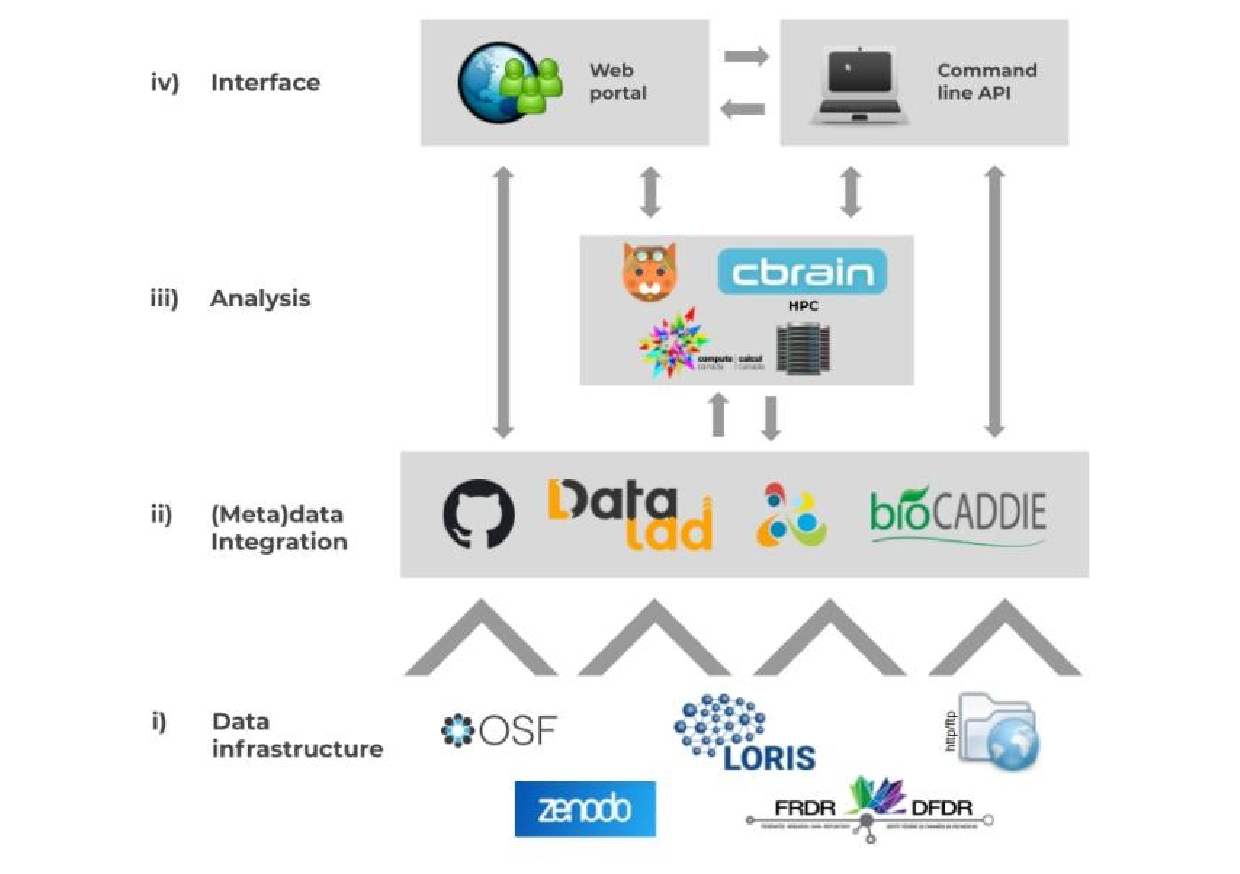
\includegraphics[width=\textwidth]{figures/CONP_figure.pdf}
    \caption{Architecture of the Canadian Open Neuroscience Platform. The platform is comprised of multiple tiers including:  i) independent data infrastructure; ii) Metadata integration across tools and datasets via standard models (Biocaddie DATS, Boutiques descriptors); iii) Data analysis on High-Performance Computing and; iv) Web and command-line interfaces. The figure is reproduced from CONP paper.}
    \label{fig:CONP_figure}
\end{figure*}

Figure~\ref{fig:CONP_figure} illustrates the architecture of CONP and since we focused on the available datasets and pipelines in CONP in our project, we explain the levels of this structure in following. 

\subsection{Data infrastructure}
CONP employes different distributed data repositories with different infrastructures, access control requirements, APIs, and licensing such as domain-agnostic datastores (OSF, Zenodo, FRDR-DFDR), specific brain imaging repositories (LORIS, XNAT, Brain-CODE), and the commonly used HTTP and FTP web protocols. Also, CONP is extensible to any repository which allows access via programmatic web-compatible interfaces.

\subsection{Data integration}
In the (meta)data integration layer, CONP leverages DataLad~\cite{datalad2021} as a backend, GitHub to host the metadata, and enables uniform data search queries based on the Data Tags Suite model~\cite{DATSDocumentation}. Datalad is responsible for integration between datasets, it is a software library for managing Git repositories referencing the data through storing metadata, file URLs and hashes of data managed by git-annex. Therefore, a DataLad dataset does not contain the data themselves, the actual datasets remain stored remotely.

Also there is a crawling framework developed in CONP which manages the life cycle of DataLad datasets on GitHub. Using this crawler as web platform, users are able to upload datasets to the CONP without knowledge of Datalad or the GitHub workflow used in CONP. This crawler searches for CONP-tagged datasets and whenever a new dataset is found creates a Datalad dataset for that, and updates the Datalad dataset whenever a modification is detected in a dataset, and then updates the CONP forked GitHub repository. Also generates DATS file with minimal information for a dataset whenever the dataset does not have one.

CONP uses CircleCI as a dataset testing suite to periodically and continuously test if datasets are available, installable by Datalad, and if data are accessible by testing the download of a few files from the datasets. To detect possible issues, CircleCI repeats such tests every four hours for all available datasets in CONP and provides a continuous monitoring for them. Also, since CONP Datalad datasets are hosted in GitHub, the integration with CircleCi would be transparent and more feasible.

\subsection{Analysis and tools}
The analysis layer not only allows finding and downloading of tools, also allows directly integrating tools into workflows and their execution on High-Performance Computing (HPC) systems such as CBRAIN~\cite{sherif2014cbrain,vaccarino2018brain}. All tools or pipelines available in CONP are described in Boutiques, which is a software library for sharing tools based on the FAIR principles. Through Boutiques library, the tools and pipelines are described as JSON objects containing the specifications about input data, parameters, and output data. 
Boutiques descriptors are also linked to a Docker or Singularity container image ``where the tool and all its dependencies are installed and configured for execution"~\cite{conp}. Tools described by Boutiques  can be published, archived, and retrieved in the Zenodo and then assigned a DOI, which makes their archives permanently findable.

\subsection{Interface}
All the technologies and methods used in CONP are described as a web portal~\cite{CONP_Portal} on which the users can search for, download and upload datasets, tools or pipelines, they are also able to lunch tools on their selected datasets using registered HPC systems such as CBRAIN without requiring advanced computing skills. 

Through the analytics available on web interface of CONP, we can see a summary of available contents. As represented in Figure~\ref{fig:cumulative}, the number of pipelines and datasets has been increased in the last three years. There are currently 57 datasets in CONP, as of July 2021. Each dataset is usually assigned a list of keywords and modalities which describes the category of compatibility of the dataset, Figure~\ref{fig:dataset_keywords} illustrates that most of the datasets in CONP are `neuroimaging'.


\begin{figure*}[ht]
  \centering
  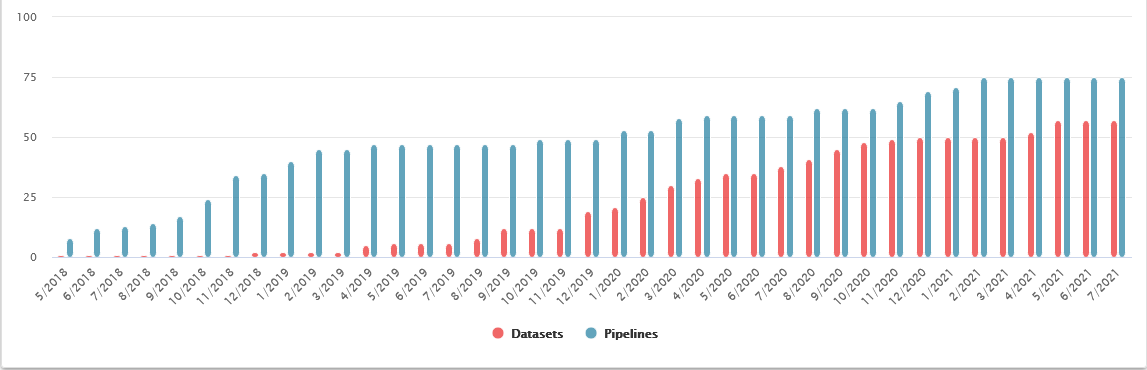
\includegraphics[width=\textwidth,height=\textheight,keepaspectratio]{figures/PipeDataTime.png}
  \caption{Cumulative number of datasets and pipelines. \\(Figure is copied form CONP portal at \url{https://portal.conp.ca/analytics})}
  \label{fig:cumulative}
  \end{figure*}

\begin{figure*}
    \centering
    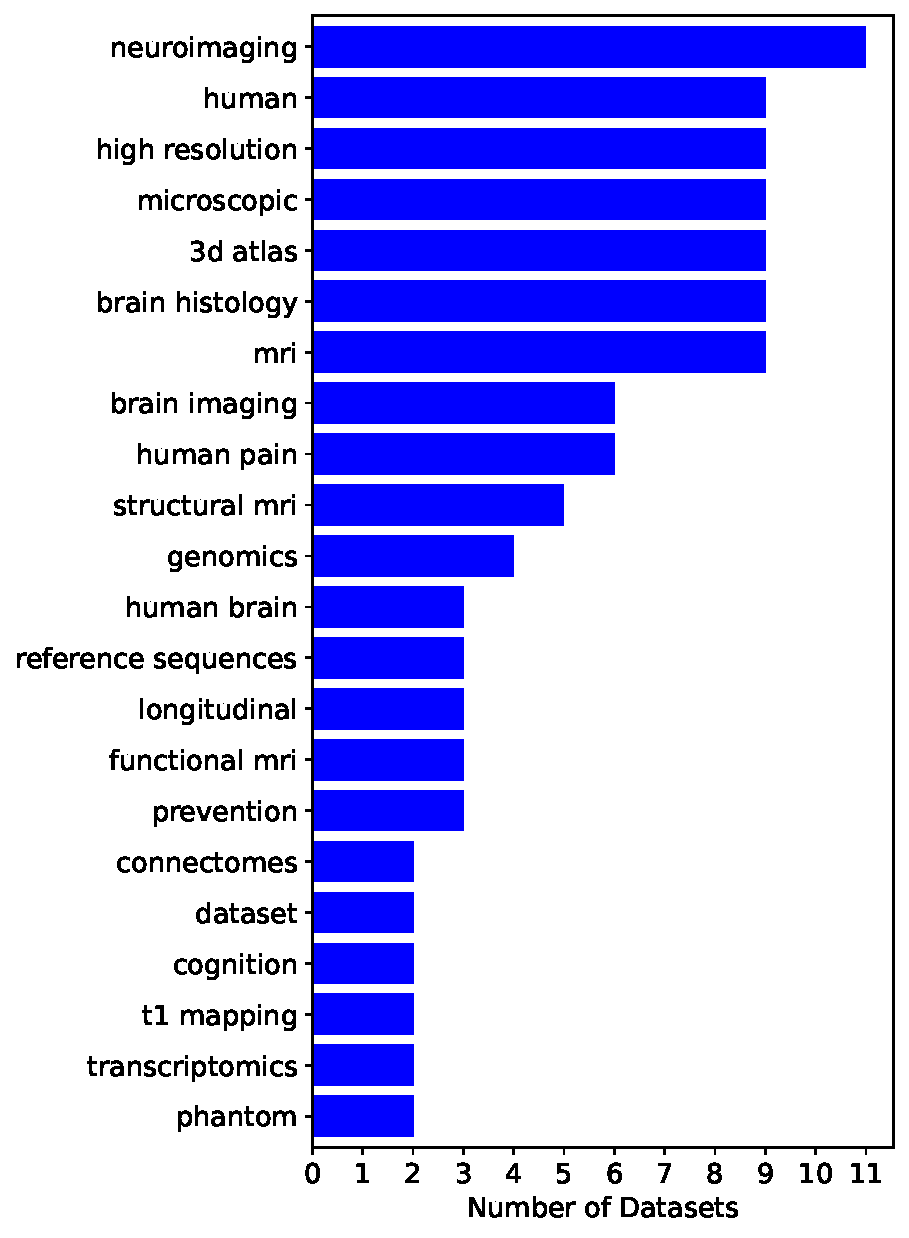
\includegraphics[width=\textwidth,height=\textheight,keepaspectratio]{figures/Datasets Keyword.pdf}
    \caption{Datasets' keywords. There have been 74 other keywords that each one is assigned to one dataset only}
    \label{fig:dataset_keywords}
\end{figure*}

\begin{figure*}
    \centering
    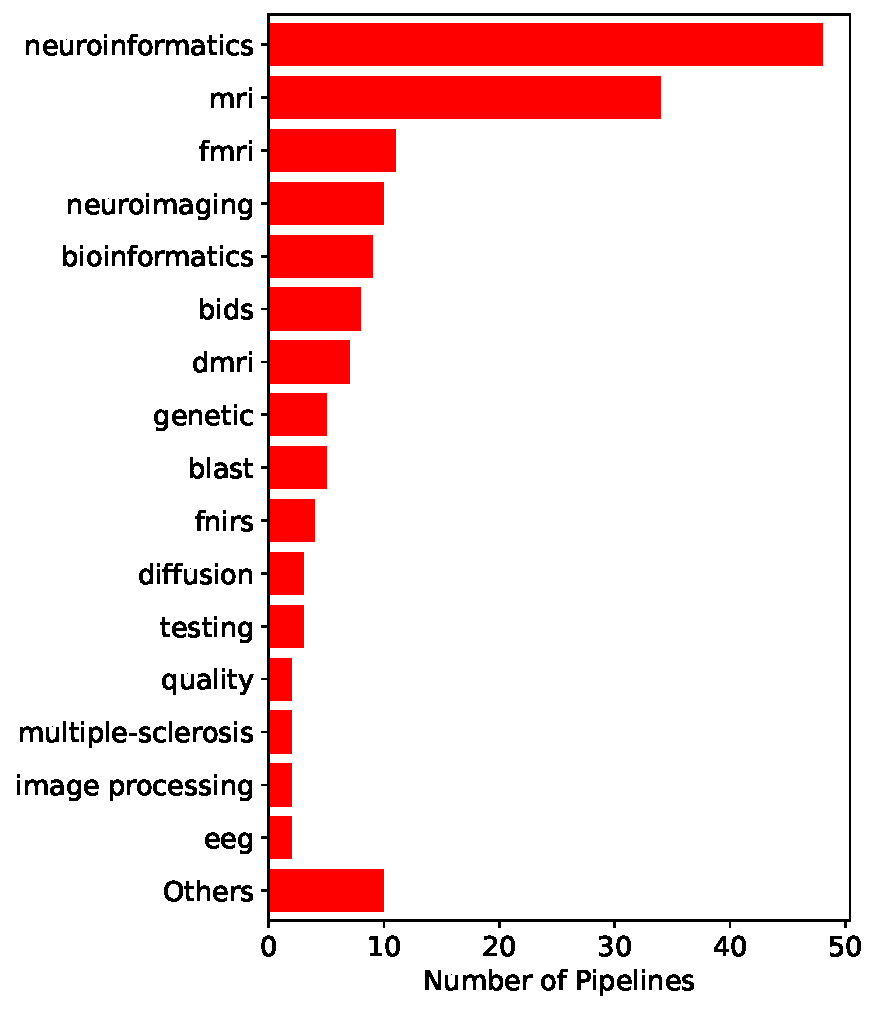
\includegraphics[width=\textwidth,height=\textheight,keepaspectratio]{figures/Pipelines Tag.pdf}
    \caption{Pipelines' tags}
    \label{fig:pipelineTags}
\end{figure*}



Also, according to Figure~\ref{fig:cumulative}, the number of pipelines has increased steadily in that period of time. Currently there are 75 tools/pipelines which many of them come from neuroscience or genomics research institutes. There are some tags assigned to each tool/pipeline which describes its category of application, as illustrated in Figure~\ref{fig:pipelineTags}, pipelines are mostly `neuroinformatics' and `mri'.







\section{Recommender Systems}

Recommender systems or recommendation systems are included in the information filtering systems which aim at providing suggestions for items to a user by predicting the `rating' or `preference' a user would give to an item~\cite{isinkaye2015recommendation,ricci2011introduction}. These suggestions might come from various decision-making processes, whether or not to buy an item, listen to a piece of music or read an article. Also, `item' is a general-purpose term referring to what the system will recommend to its users. For instance, it can be a software tool, news or magazine, and products to purchase. The definitions provided in the rest of this section are mostly a summary of Chapter 9 of~\cite{rajaraman2011mining}.

Currently, the recommender systems can be seen anywhere that a possible user needs to choose an `item.' From the most popular recommendation systems, we can point to product recommendations, movie recommendations and news and article recommendations. In product recommendations, online retailers such as Amazon are increasingly attempting to attract and keep their users by suggesting more relevant products that they might like to buy. This will lead to a win-win outcome, finding relevant products for the users and increasing the revenue for the business owners. 

Another application of recommender systems is movie recommendations such as Netflix, which recommends to its users the movies or TV shows that they might like based on many factors such as previously watched movies, the ratings (currently `like' or `dislike') given or the similar users' choices. There are so many other factors that help Netflix to provide good suggestions for its users. Another application of recommender systems can be in news and articles in which the goal is to identify articles that users would like to read based on what they have read before.





There are several technologies in recommender systems to find the best `item' for a `user' that we can classify in two broad groups, Content-based and Collaborative filtering \cite{rajaraman2011mining}. A content-based recommender system focuses on an item/user profile which describes a set of features and properties of that item/user. Then recommends an item to a user if it is similar to the previous choices of the user. However, a Collaborative filtering recommender system focuses on the relationship between users and items; items will be recommended to a user if similar users prefer it. 

Before going through detailed explanations of Content-based and Collaborative Filtering recommendation approaches, we need to define the Utility Matrix and its role in recommendation approaches. 
\subsection{Utility Matrix}
In the recommender systems, `user' and `item' are the terms used to represent the two main classes of entities.  The Utility Matrix is indexed with users' ids on one axis and items' on the other and includes values assigned to each user-item pair, representing the user's preference for the item. In this case, values might represent the item's rating given by the user, 1-5 stars, for example. Usually, the utility matrix is sparse, meaning that the rating value for most user-item pairs is `unknown,' which implies that there has not been explicit information about the user's preference for that item. 
%, or the number of times a user has selected the item ( >= 0), for instance, the number of downloads, views or buying an item.

Figure~\ref{fig:utilityMatrix} is an example in which the utility matrix represents the ratings (1-5) for movies (HP1, HP2, and HP3 for Harry Potter I, II, and III, TW for Twilight, and SW1,
SW2 and SW3 for Star Wars episodes 1, 2, and 3) given by the users (A, B, C, D). The blank units represent unknowns, in which the user has not rated the movie. In practice, the utility matrices are mostly sparser than this matrix since a small fraction of real users gives explicit feedback on items. The goal of the recommender system is to predict the value for the blanks in the utility matrix.

% We should also be aware of a slightly different goal that makes sense in
% many applications. It is not necessary to predict every blank entry in a utility
% matrix. Rather, it is only necessary to discover some entries in each row that
% are likely to be high. In most applications, the recommendation system does
% not offer users a ranking of all items, but rather suggests a few that the user
% should value highly. It may not even be necessary to find those items with
% the highest expected ratings, but only to find a large subset of those with the
% highest ratings.

\begin{figure*}[ht]
  \centering
  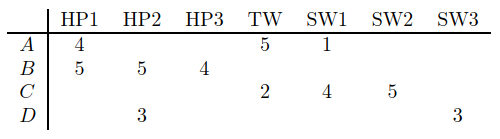
\includegraphics[width=\textwidth]{figures/utilityMatrix.png}
  \caption{A utility matrix representing ratings of movies on a 1–5 scale. Figure extracted from Chapter 9 of~\cite{rajaraman2011mining}}
  \label{fig:utilityMatrix}
\end{figure*} 


The utility matrix is the most important requirement to generate a recommendation system. However, it is usually difficult to acquire data from users for the utility matrix. There are two general approaches to gather data from users, first by asking them to rate the items. For instance, asking them to rate after watching a movie or buying a product. However, this this approach is not effective due to the fact that users usually are not willing to provide responses, so the collected information might be biased since it is provided by people who are willing to give ratings. Another approach would be data acquisition from users interactions and behaviour. For instance, if a user
buys a product, watches a movie, or reads an article, it represents that they `liked' that item. For this sort of rating the only value is 1 (for getting user's response) and the unknown pairs would be 0; in this case 0 is not lower that 1, it is no rating at all.


\subsection{Implicit and explicit feedback data}

Recommender systems rely on different types of input data which are categorized as explicit feedback and implicit feedback.
The explicit feedback which is more convenient one, includes the ratings, or any other types of inputs which the users have provided explicitly, such as the stars representing movie rating. However, explicit feedback is not always available and should be captured from investigating the behavior of user which indirectly reflect their preferences such as purchase history, browsing history, search patterns, or even mouse movements~\cite{hu2008collaborative}. The majority of the literature related to recommender systems are focused on explicit feedback, however, in many practical situations it is required to consider the implicit feedback data. 

There are some unique characteristics for implicit feedback data  which prevent the direct use of algorithms that are designed for explicit feedback. First, there is no negative feedback, since the implicit data is based on user's behaviours, it is not possible to understand which items the user does not like. For example, not watching a movie does not necessarily mean that the user does not like it, it probably means that they did not know about that, or did not have access to that. In this case, the user-item pairs that there is no gathered data for, usually the vast
majority of the data, are treated as “missing data” and will be omitted from the analysis. 

Second characteristic is that implicit feedback data are noisy, meaning that the user-item interactions do necessarily mean the user's preference. For instance purchasing might be as a gift, or the user might be unhappy after using that. Third, numerical values in implicit feedback data describe the frequency of actions not user's preference, for instance, how many times a certain movie is watched by a user, or a certain product is ordered by a user. In this case a larger value does not mean a higher preference.
``For example, the most loved show may be a movie that the user will watch only once, while there is a series that the user quite likes and thus is watching every week"~\cite{hu2008collaborative}. 

And finally, evaluation of implicit-feedback recommenders is more sophisticated than for the explicit feedback. When the items are explicitly scored by the user, clear metrics such as mean square error can be used to measure the success rate of predictions. However,there are many factors to be considered for implicit feedback such as the availability of the item, the repeat feedback, and the competition for an item among others. For instance, the user might have to choose one program among two of his/her favourite shows that will be played at the same time.

\subsection{Content based}
Content-based recommender systems focus on the item's properties described in its profile and then recommends a user the similar items to the ones they `liked' before. The profile for an item or user is a set of properties or descriptions assigned to item or user. Similarity between items will be obtained by measuring the similarity between their profiles. 


The item profile consists of item's properties, there are different classes of items and for each class of them the approach for collecting the properties is different. The first and most convenient way of obtaining features is when the features are explicitly assigned to the item. For instance, the movies usually are assigned with the number of stars indicating the level of users' preference, and other properties such as year of production, name of director and actors and the genre. Another example can be the products which usually are described by the manufacturer with relevant features. 

There are other classes of items which the values of features are not immediately apparent, such as documents. Documents, articles and web pages, consist of thousands of words but do not tend to have readily available assigned information to be used to find their topic. To characterize this class of items, it is required to remove the stop words (such as `is',`they') and then compute the TF.IDF score~\cite{ramos2003using} for all remaining words, the top n words with highest scores will characterize the document.


In content-based recommendation, there should be item profile and user profile~\cite{rajaraman2011mining}. Item profile consists of feature-value pairs and user profile summarizes the preferences of the user. There would be a feature matrix with columns that are features, the values for features can be Boolean or numerical, each row represents an item's profile as a vector of its features. The user profile should represent the preference of the user about items, which can be achieved by aggregation of the profiles of items which user has `liked'. Then for estimating the degree to which a user would prefer an item, the cosine distance between the user’s and item’s vectors should be computed, the less distance represents the more chance of preference.

% "If the utility matrix has only 1’s, then the natural aggregate is the average of the components of the vectors representing the item profiles for the items in which the utility
% matrix has 1 for that user. If the utility matrix is not Boolean, e.g., ratings 1–5, then we can weight the vectors representing the profiles of items by the utility value. It makes sense to normalize the utilities by subtracting the average value for a user. That way, we get negative weights for items with a below-average rating, and positive weights for items with above-average ratings"~\cite{rajaraman2011mining}.



\subsection{Collaborative filtering}
Collaborative filtering is one of the most successful approaches for recommender systems which identifies new user-item associations by analyzing the relationships between users and interdependencies among items (products)~\cite{koren2009matrix}. The fundamental assumption of Collaborative Filtering is that users with similar preferences in the past are likely to have similar preferences in the future~\cite{su2009survey}. ``A major appeal of collaborative filtering is that it is domain free, yet it can address data aspects that are often elusive and difficult to profile using content filtering"~\cite{koren2009matrix}. There are three main categories of Collaborative Filtering, Memory-based, Model-based and Hybrid collaborative filtering (which combines Collaborative Filtering with other techniques). 

In Memory-based Collaborative Filtering algorithms the assumption is that every user is from a group of users with similar interests. Therefore prediction of preferences of a new user on a new items can be produced by identifying the neighbors of that user.
Neighbor-based collaborative filtering (kNN) is the prevalent algorithm in this class. 
Although memory-based Collaborative Filtering approaches are identified as easy-to-implement and highly effective, they have many limitations including the fact that user-item ratings should be stored in memory, adding a new items is sophisticated, and the performance decreases when the data is sparse since the similarity values are based on common items.


To overcome the limitations of memory-based collaborative filtering and providing better performance, the model-based collaborative filtering was investigated~\cite{su2009survey,la2021evaluating}. Model-based collaborative filtering techniques use the pure rating data to learn/train a model which can later be used for predictions. In this class the model can be data mining or machine learning algorithms. Also, since it is not required to have data stored in memory, the prediction process can be fast and even using less data than the original. Among the possible techniques, the Latent Factor based algorithms are proven to be effective to address the scalability and sparsity challenges of collaborative filtering tasks.



Among the techniques for latent factor models, some of the most successful ones are based on matrix factorization~\cite{koren2009matrix} which aims to extract meaningful latent connections between users and items based on user-item rating patterns. Recommender models based on Matrix factorization ``map both users and items to a joint latent factor space of dimensionality $f$, such that user-item interactions are modeled as inner products in that space". Each item $i$ is associated with a vector of factors (features) 
$q_{i}\in \mathbb{R}^{f}$
which represents how much (positive or negative) this item contains those factors; similarly, each user $u$ is associated with a vector of factors(features) 
$p_{u}\in \mathbb{R}^{f}$
which measure the extent of interest the user has in items that are high on the corresponding factors. 


To learn the latent factors ($p_{u}$ and $q_{i}$), more recent works suggested modeling based on the known ratings, therefore, the regularized squared error should be minimized on the set of 
known ratings:
\begin{equation} \tag{1}
   \min_{q_{*},p_{*}} \sum_{(u,i) \epsilon \kappa }  (r_{ui}-q_{i}^{T}p_{u})^{^2}+\lambda \left ( \left \| q_{i}\right \|^2+\left \| p_{u}\right \|^2 \right )            \label{equation}
\end{equation}
where $\kappa$ is the set of user-item pairs for which $r_{ui}$, the rating of item $i$ by user $u$, is available. Unknown elements of the utility matrix are predicted by the value of $q_{i}^{\tau }p_{u}$ which represents the user’s overall interest in the item’s characteristics and is an approximation of the rated value if item $i$ by user $u$. 


\subsection{Content-based and Collaborative Filtering in our context}

As mentioned before, we aim at recommending the compatible datasets and analysis pipelines available in CONP. To have a content-based recommender approach we should focus of ....

Also there is concept as "automated metadata generation" which works as... however currently this is not implemented for the pipeline/datasets in CONP and would be a much large and complicated for us to implement in a master project....

Therefore we focused on Collaborative filtering which would be .....
